\subsection{Data} \label{subsec:data_linear_regression}
In this project, we are fitting $2D$ polynomials to the Franke function for different values of the noise. The Franke function is defined as
\begin{equation}
    \begin{split}
        f(x_1,x_2) := \frac{3}{4}\exp{\left(-\frac{(9x_1-2)^2}{4}-\frac{(9x_2-2)^2}{4}\right)} \\ + \frac{3}{4}\exp{\left(-\frac{(9x_1+1)^2}{49}-\frac{(9x_2+1)}{10}\right)} \\+ \frac{1}{2}\exp{\left(-\frac{(9x_1-7)^2}{4}-\frac{(9x_2-3)^2}{4}\right)} \\ - \frac{1}{5}\exp{\left(-(9x_1-4)^2-(9x_2-7)^2 \right)}
    \end{split}
\end{equation}
To this Franke function, we add noise sampled from a Gaussian distribution $\mathcal{N}(0, var)$ to get a noisy Franke function:  $\tilde{f}(x_1,x_2)$. 
\begin{figure}
\centering
\begin{subfigure}{.5\textwidth}
  \centering
  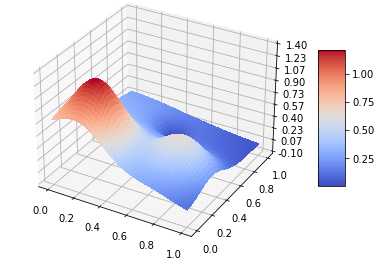
\includegraphics[width=.9\linewidth]{Images/franke_function.png}
  \caption{}
  \label{fig:franke}
\end{subfigure}%
\begin{subfigure}{.5\textwidth}
  \centering
  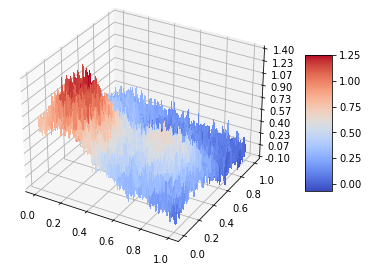
\includegraphics[width=.9\linewidth]{Images/franke_function_noise.png}
  \caption{}
  \label{fig:franke_noise}
\end{subfigure}
\caption{Plot of the Franke function with noise (b) and without noise (a). The variance of the added noise is 0.1.}
\label{fig:franke_function}
\end{figure}